
%%%%%%%%%%%%%%%%%%%%%%% file typeinst.tex %%%%%%%%%%%%%%%%%%%%%%%%%
%
% This is the LaTeX source for the instructions to authors using
% the LaTeX document class 'llncs.cls' for contributions to
% the Lecture Notes in Computer Sciences series.
% http://www.springer.com/lncs       Springer Heidelberg 2006/05/04
%
% It may be used as a template for your own input - copy it
% to a new file with a new name and use it as the basis
% for your article.
%
% NB: the document class 'llncs' has its own and detailed documentation, see
% ftp://ftp.springer.de/data/pubftp/pub/tex/latex/llncs/latex2e/llncsdoc.pdf
%
%%%%%%%%%%%%%%%%%%%%%%%%%%%%%%%%%%%%%%%%%%%%%%%%%%%%%%%%%%%%%%%%%%%


\documentclass[runningheads,a4paper]{llncs}

% pour les accents utilisés en français 
\usepackage[utf8]{inputenc}
\usepackage[T1]{fontenc}
\usepackage[french]{babel}
\usepackage[hiperref]{}

%\usepackage{amssymb}
\setcounter{tocdepth}{3}

%images config
\usepackage{graphicx}
\graphicspath{ {images/} }

% for matrixes
\usepackage{amsmath}

\usepackage{url}
\urldef{\mailsa}\path|samuel.carensac@insa-lyon.fr|    

\begin{document}

\mainmatter  % start of an individual contribution

% first the title is needed
\title{Contrôle du mouvement sur support\\ mou ou liquide}

% a short form should be given in case it is too long for the running head
\titlerunning{Lecture Notes in Computer Science: Authors' Instructions}

% the name(s) of the author(s) follow(s) next
%
% NB: Chinese authors should write their first names(s) in front of
% their surnames. This ensures that the names appear correctly in
% the running heads and the author index.
%
\author{Samuel Carensac}
%
\authorrunning{Lecture Notes in Computer Science: Authors' Instructions}
% (feature abused for this document to repeat the title also on left hand pages)

% the affiliations are given next; don't give your e-mail address
% unless you accept that it will be published
\institute{Université de Lyon 1,\\
\mailsa}

%
% NB: a more complex sample for affiliations and the mapping to the
% corresponding authors can be found in the file "llncs.dem"
% (search for the string "\mainmatter" where a contribution starts).
% "llncs.dem" accompanies the document class "llncs.cls".
%

\toctitle{Lecture Notes in Computer Science}
\tocauthor{Authors' Instructions}
\maketitle


\begin{abstract}
 L'animation basée physique est de plus en plus étudiée car elle permet de réaliser les interactions avec l'environnement beaucoup plus simplement. Bien qu'il existe des contrôleurs permettant la simulation des interaction d'un personnage en milieu liquide ceux-ci ne se sont que la nage. Nous présentons une stratégie de contrôle de mouvement d'un personnage virtuel en immersion partielle dans un liquide. L'effet des liquides sur le mouvement du personnage est modélisé à l'aide de formules d'hydrodynamiques simples. Notre contrôleur permet de combiner différents styles de marches, d'assurer l'équilibre par le placement intelligent du pied et d'assurer le contrôle précis de la vitesse du personnage. Le controler a été test dans une situ de manche dans un niveau d'eau. dire que on a  fait de l'opti sur 4 niveau. 
A la suite de cette optimisation nous avons obtenu un contrôleur capable de s'adapter automatiquement à ..... une quantité de liquide, variation de densité, variations de vitesses désirée...
\keywords{*We would like to encourage you to list your keywords within
the abstract section*}
\end{abstract}

\section{Introduction}
%
La simulation de mouvements humains réaliste est un point clef dans la création d'un environnement virtuel.*faire une phrase qui dit ce qu'est un monde complexe et une disant comment l'anim ciné gère les interactions dire que historiquement on a util la ciné en prems*.   Les mondes virtuels étant de plus en plus complexes il est devenu difficile d'arriver à réaliser des interactions réalistes entre les personnages animés et l'environnement à l'aide des méthodes d'animation cinématique. *dire que les anim physique util des force et pk ça permet de bien avoir les interactions* Un nombre grandissant de travaux se portent maintenant sur la création de contrôleurs basés physiques. Bien que ceux-ci permettent d'obtenir naturellement les interaction avec l'environnement, la manipulation du personnage devient bien plus complexe car l'on a pas de contrôle direct sur la position des membres des personnages animés.

Le défi principal d'un contrôleur physique est de permettre la paramétrisation haut niveau du système. Ces paramètres peuvent être vitesse, heading, .... Le besoin de simuler un très grand nombre de styles de déplacement (marche, course, saut, ...) rend la création d'un contrôleur générique extrêmement difficile. De même la maitrise des interactions avec l'environnement ajoute également une très grande complexité au système. C'est pourquoi les contrôleurs existants se concentrent sur l'étude d'un nombre limité de styles de déplacement et d'interactions avec l'environnement *ref à l'état de l'art*. Les travaux que nous présentons dans ce document se focalisent sur le contrôle de la marche dans des conditions d'immersion partielle du bas du corps dans un liquide.*l'objectif scientifique que nous nous somme fixé est de def et d'implémenter les mécanismes nécessaire à un contrôler physique permettant l'anim temps réel d'un perso virtuel en interaction avec un liquide* . Notre contrôleur est également capable d'une grande liberté de style de marche et d'un contrôle précis de la vitesse de déplacement du personnage.

Notre stratégie de contrôle s'inspire de plusieurs contrôleurs existants. Notre système est composé de cinq composants clefs. Le premier est une modélisation des effet des liquides sur le personnage à l'aide de formulation de concepts d'hydrodynamique.
Le second est un système permettant d'interpoler plusieurs trajectoires cibles en fonction de la vitesse désirée. Le troisième permet l'adaptation du contrôle du mouvement pour de prendre en compte l'influence du liquide.  Le quatrième consiste à planifier le mouvement de la jambe en phase de vol. Le dernier gère le contrôle précis de la vitesse et de l'équilibre.

Finir par le plan du document (mettre des voir dnas le paragraphé précédent)
mettre le plan général sans rentrer dnas les sous sections

%%%%%%%%%%%%%%%%%%%%%%%%%%%%%%%%%%%%%%%%%%%%%%%%
%%%%%%%%%%%%%%%%%%%%%%%%%%%%%%%%%%%%%%%%%%%%%%%% 

%
\section{État de l'art}
%
\subsection{Animation de personnages humains} 
Pour pouvoir réaliser l'animation d'un personnage, il est nécessaire de disposer d'une structure représentant ce dernier. La structure la plus utilisée est un squelette modélisation du personnage utilise divers corps rigide reliés par des articulations. Chaque articulation dispose de un à trois degrés de liberté de rotation sur lesquels pourront être appliqués des moments. *expliquer coment le moment modifie l'angle $\tau=\alpha_i$* . Des limites sont mises en place sur les articulations (angles maximums, moments maximum) pour représenter les limites anatomiques du personnage. 
%metre ces truc en intro
%Il existe deux catégories de méthodes d'animation. La première, l'animation cinématique, décrit simplement les trajectoires des articulations au cours du %temps. Bien que facile à réaliser cette méthode possède le défaut de rendre les interactions avec un environnement dynamique très compliquées. La %seconde catégorie, l'animation basée physique, aborde le problème sous un tout autre angle.
 En animation physique On peut classer les interfaces de contrôle du squelette en trois catégories \cite{geijtenbeek2012interactive}:
\begin{itemize}
\item{Dans la première, le squelette est animé par l'application de moments aux des articulations.}
\item{La seconde consiste à appliquer des forces externes directement sur les différents corps solides pour les déplacer. Ces forces n'ayant pas d'équivalent dans la réalité, les mouvements obtenus peuvent ne pas sembler naturels. Cette technique a d'ailleurs été surnommé "hand-of-god" \cite{van1995guided}. }
\item{La dernière consiste à simuler des forces externes à l'aide de moments appliqués aux articulations. Ce type de forces est appelé forces virtuelles.}
\end{itemize}

En raison du grand nombre de données nécessaires pour produire une animation, l'utilisation directe de ces méthodes est prohibitive. C'est le rôle du contrôleur de générer ces données à partir de paramètres haut niveau. Ces paramètres doivent être intuitifs pour l'utilisateur tels que vitesse et direction du mouvement \cite{coros2010generalized}. 

\subsection{Contrôle dans l'espace des articulations} 
Le type de contrôleur le plus commun utilisant les 3 interfaces citées précédemment se dénomme "Contrôleur dans l'espace des articulations".
De manière similaire à l'animation cinématique, ce type de contrôleur utilise une série de poses désirées représentant le mouvement à reproduire. La Figure \ref{fig:joint_space_motion_control} (à gauche) présente une vue d'ensemble d'un tel contrôleur. Le bloc "balance and pose control" a pour rôle de convertir les paramètres choisis par l'utilisateur en une cible cinématique définissant les angles et le vitesses pour chaque articulation. Ces paramètres peuvent être de haut niveau (vitesse, hauteur des pas) ou des poses de références. Le bloc "local feedback control" calcule les moments nécessaires pour atteindre la pose désirée pour chaque articulation. Ce bloc permet d'intégrer des mécanismes de calcul de moments supplémentaires (e.g. pour le contrôle de la vitesse). 
\begin{figure}[h]
\centering
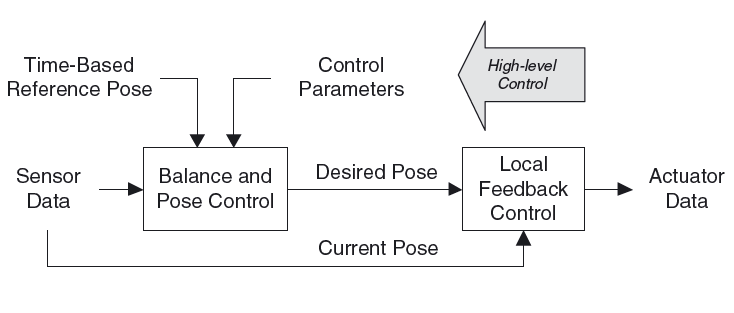
\includegraphics[scale=0.4]{joint_space_motion_control.png}
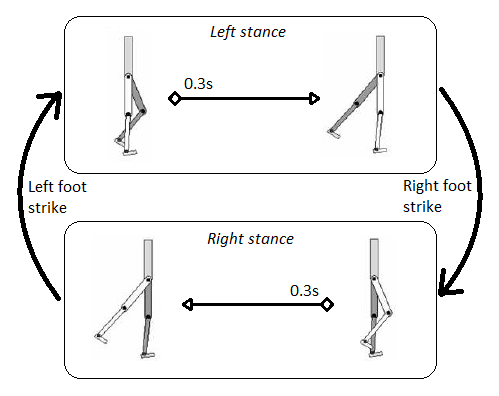
\includegraphics[scale=0.5]{state_machine.png}
\caption{A gauche, exemple de contrôleur dans l'espace des articulations \cite{geijtenbeek2012interactive}. A droite, exemple de machine à état pour la marche \cite{yin2007simbicon}}
\label{fig:joint_space_motion_control}
\label{fig:state_machine}
\end{figure}



Bien qu'il existe plusieurs méthodes permettant de suivre les poses désirées (antagonist feedback \cite{neff2002modeling}, non-linear force field \cite{mussa1997nonlinear}), la méthode la plus commune est le "proportionnal-derivative control" (PD-control). Un PD-contrôleur calcule un moment  \(\tau\) pour chaque articulation proportionnel à la différence entre l'état actuel et l'état désiré. Il prend en compte non seulement la différence entre les angles mais aussi la différence entre les vitesses angulaires. 
\begin{equation}
\tau=k_p(\theta_d - \theta) + k_v(\dot{\theta_d} - \dot{\theta})
\label{eq:pd_controler}
\end{equation}
Avec \(\theta_d\) et \(\dot{\theta_d}\) l'angle et la vitesse désirée, \(\theta\) et \(\dot{\theta}\) l'angle et la vitesse courante et \(k_p\) et \(k_v\) des constantes de vitesse et de position appelées les gains du PD-contrôleur.
Parmi les systèmes basés sur un PD-contrôleur on trouve notamment le SIMBICON (SIMple BIped CONtroler) \cite{yin2007simbicon}. Ce système est basé sur une machine à état fini. Chaque état est défini par une série de poses clefs qui définissent les poses désirées au cours du mouvement. La transition d'un état à un autre peut s'effectuer après un certain temps ou bien lors d'un nouveau contact entre un pied et le sol. La figure \ref{fig:state_machine} (droite) illustre la composition d'un contrôleur SIMBICON pour la marche. La spécification des poses clefs des états possèdent quelques spécificités propres au SIMBICON. Les angles des articulations sont exprimés dans un repère local à l'exception de l'articulation entre le bassin et le dos et de celle de la hanche en phase de vol. Enfin la hanche d'appui ne possède pas de positions cibles. Le moment \(\tau_b \) à appliquer à la hanche d'appui est calculé de manière à ce que le moment total sur le pelvis corresponde au moment \(\tau \) permettant d'obtenir l'orientation définie par l'utilisateur. Ce moment \(\tau \) désiré est déterminé par le PD-contrôleur en prenant pour angle cible la somme de l'angle définit dans la trajectoire du pelvis plus l'angle de direction du mouvement (figure \ref{fig:torques_pelvis}).
\[
\tau_b=\tau - \tau_a - \tau_{torso}
\]
Avec \(\tau_a \) le moment appliqué sur la hanche de balance et \(\tau_{torso} \) le moment appliqué à l'articulation entre le pelvis et le torse.


\label{sec:jacob}
\begin{figure}[h]
\centering
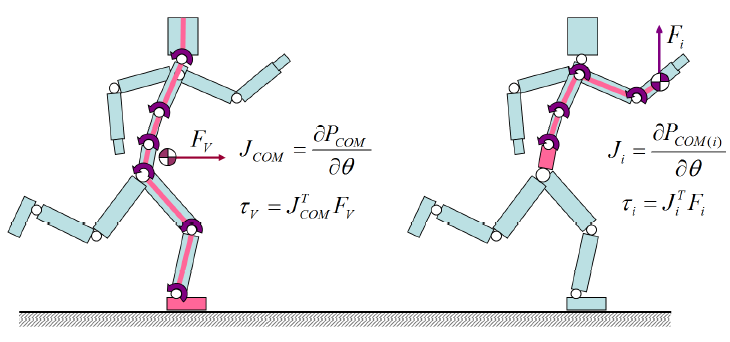
\includegraphics[scale=0.5]{shema_jacobians.png}
\caption{A gauche, jacobienne utilisée pour le contrôle de vitesse. A droite, jacobienne utilisée pour la compensation de gravité. \cite{coros2010generalized} }
\label{fig:jacob}
\end{figure}

Le défaut du PD-contrôleur est qu'il est nécessaire de connaitre les bonnes valeurs pour les gains si l'on veut obtenir un résultat correct. Des gains trop bas ne permettraient pas de suivre le mouvement définit. Des gains trop élevés provoqueraient un mouvement saccadé et des possibles oscillations autour de la position désirée. On peut déterminer les paramètres optimaux pour une configuration (mouvement, géométrie du personnage, interaction avec l'environnement, ...) par une série d'essais successifs mais le contrôleur obtenu ne serait pas robuste aux variations de configuration et entrainerait des déséquilibres. Pour pallier ce problème SIMBICON utilise un système de feedforward \cite{yin2007simbicon} qui permet d'apprendre une partie des moments nécessaires. Les PD-contrôler n'étant plus utilisés pour les calculs, des gains bas sont suffisant. 
L'extension du SIMBICON proposé par \cite{coros2010generalized} présente un système de compensation de gravité permettant également de calculer une partie des moments nécessaires. Le principe est de calculer pour chaque partie du personnage une force virtuelle compensant la gravité. Donc pour chaque membre du personnage une force virtuelle \(F_{GC}=-mg\) est appliquée au centre des masses, le signe négatif indiquant une force vers le haut. Cette force est ensuite convertie en moment pour chaque articulation se trouvant dans la chaine reliant le point d'application de la force et le pelvis \(\tau=J_i^T F\); où \(J_i ^T\) est la transposée de la jacobienne de la chaine reliant le pelvis et le point d'application de la force. La figure \ref{fig:jacob} droite illustre la chaine affectée par la compensation de gravité d'un bras.
La jacobienne d'une chaine de \(k\) articulations contient les informations indiquant l'impact d'une rotation de chaque degré de liberté de la chaine sur la position du point d'application de la force. Chaque $J(p)_i ^T$ peut être calculé par le produit vectoriel entre l'axe de la rotation $\alpha_i$ et le vecteur allant de l'articulation \(i\) et le point d'application $p$.
\[
J_i ^T (p)=\begin{bmatrix}
\frac{\partial p_x}{\partial \alpha_i} & \frac{\partial p_y}{\partial \alpha_i} & \frac{\partial p_z}{\partial \alpha_i} \\
\end{bmatrix}
= (\alpha_i \times (p-p_i))^T
\]
Donc la force à appliquer à chaque articulation i correspond à:
\[
\tau = (\alpha_i \times (p-p_i))^T F
\]
Cette méthode de compensation de gravité est appliquée à tous les membres du squelette excepté ceux composant la jambe d'appui.


\subsection{Maîtrise de l'équilibre au cours de la marche}

Tel qu'il est définit, le système permet d'effectuer un mouvement pour la configuration apprise. Cependant toute perturbation, même minime, peut provoquer une perte d'équilibre du personnage.

\begin{figure}[h]
\centering
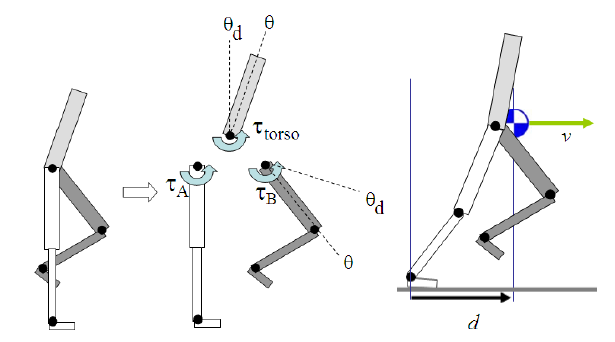
\includegraphics[scale=0.5]{stance_torque_and_v_and_d.png}
\caption{A gauche, calcul des moments sur le pelvis \cite{yin2007simbicon}. A droite, représentation des variables \(d\) et \(v\) \cite{yin2007simbicon}.}
\label{fig:torques_pelvis}
\label{fig:d_and_v}
\end{figure}

Pour pallier ce problème le SIMBICON ajoute un système de balance feedback sur la hanche en phase de vol et le pied d'appui. Le principe est de modifier les angles cibles en fonction de la vitesse $v$ du centre des masses du personnage et de la distance \(d\) séparant celui-ci et le pied d'appui (voir figure \ref{fig:d_and_v} droite). 
\[
\theta_d=\theta_{d0} + c_d*d + c_v*v 
\]
Avec \(\theta_d\) l'angle qui sera utilisé par le PD-contrôleur et \(\theta_{d0}\) l'angle spécifié par l'utilisateur.
Les gains \(c_d\) et \(c_v\) sont déterminés pendant la phase d'optimisation hors-ligne. Il est important de signaler que la nécessité d'avoir des gains optimaux la rend très peu flexible.


Parmi les autres systèmes de placement intelligent du pied on trouve l'utilisation d'un modèle du pendule inversé (IPM) \cite{coros2010generalized,kajita20013d}.L'avantage majeur de l'IPM est qu'il est totalement autonome et ne nécessite pas de configuration manuelle ou d'optimisation offrant ainsi une grande robustesse aux perturbations. Cette version de l'IPM considère une longueur de jambe constante. Le principe de l'IPM est de partir du constat que la somme de l'énergie potentielle de pesanteur et de l'énergie cinétique reste constante peu importe la position du pendule  $\frac{1}{2}mv^2+mgh=\frac{1}{2}mv'^2+mgh'$ (figure \ref{fig:ipm}).La supposition d'une vitesse nulle lors de la position d'équilibre (position verticale) nous permet de simplifier l'équation avec les variables suivantes \(v'=0\) et \(h'=L=\sqrt{h^2+d^2}\). On peut ainsi déterminer la position \(d\) du prochain posé de pied nous permettant d'obtenir un état d'équilibre.
\[
d=v\sqrt{\frac{h}{g}+\frac{v^2}{4g^2}}
\]
Selon la vitesse du personnage il est possible que l'IPM nous donne des résultats impossible à atteindre c'est pourquoi la longueur des pas est limitée à \(d=0.6L\) avec \(L\) la longueur de la jambe.
Pour permettre d'avoir un résultat conservant une vitesse proche de la vitesse désirée \(V_d\) une altération $\delta$ des résultats de l'IPM est réalisée en utilisant la loi suivante \(\Delta=\alpha V_d\), $\alpha$ étant une constante négative. Ainsi une vitesse positive apporte une diminution de la longueur des pas provoquant une accélération du personnage et inversement une vitesse négative ralentit le personnage.
La position effective du pied est calculée à l'aide d'une interpolation entre la position de départ du pied et la valeur retournée par l'IPM. La loi d'interpolation utilisée est une loi d'ordre 2:
\[
P_f=(1-\phi^2)*pos_{init}+\phi^2*p(x,y)
\]
La hauteur du pied au cours du pas est définie par l'utilisateur à l'aide d'une trajectoire.
Les angles désirés pour la hanche et le genou sont ensuite déterminés à l'aide de la cinématique inversé. Il reste un degré de liberté qui peut être contrôlé par l'utilisateur.

En plus de permettre l'équilibre l'IPM possède l'avantage de pouvoir complètement définir le mouvement de la jambe en phase de vol pour la marche humaine en utilisant des paramètres plus haut niveau tel que la hauteur des pas et la vitesse désirée. Un avantage majeur d'un tel système est que l'on obtient une définition indépendante des caractéristiques physique du squelette offrant ainsi une grande flexibilité. Cependant, bien que l'IPM soit très performant, son utilisation limite le déplacement à de la marche car il suppose un contact permanent avec le sol. De plus, l'utilisation d'un IPM pour générer le mouvement complet de la jambe en phase de vol limite grandement les styles de déplacement possibles. En effet il est impossible de déplacer le pied verticalement sans le déplacer dans le plan horizontal.

\subsection{Contrôle de la vitesse}
Parmi les paramètres de haut niveau primordiaux disponibles à l'utilisateur on trouve la vitesse. Dans la version originale du SIMBICON le respect d'une vitesse désirée est obtenu à l'aide d'une stratégie d'évolution. Le principe est de faire varier les poses clefs jusqu'à ce que l'on obtienne un mouvement avec la vitesse voulue. Le défaut est que non seulement il est nécessaire de trouver les poses clefs pour chaque vitesse désirée mais il est également impossible de faire varier la vitesse sans arrêter la simulation. Une amélioration du contrôleur \cite{coros2009robust} apporte la possibilité d'avoir plusieurs états. Le principe est d'avoir des généraux (i.e. marche avant, marche arrière, …) et de faire des combinaisons de ces états pour obtenir des états intermédiaires. Cela permet de changer de vitesse sans avoir à arrêter la simulation et diminue le nombre de poses clefs nécessaires pour obtenir de multiples vitesses. Cependant, ce système n'assure qu'un suivit peu précis de la vitesse désirée si l'on s'éloigne des états définis.
Plus récemment, une méthode se servant d'une force virtuelle horizontale pour accélérer ou ralentir le personnage a été présentée \cite{coros2010generalized}. Le principe est d'appliquer une force virtuelle sur le centre des masses du personnage pour créer une déséquilibre vers l'avant ou vers l'arrière permettant de contrôler la vitesse du personnage. L'intensité de la force à appliquer est calculée à l'aide d'un PD-contrôler se basant sur la différence entre la vitesse courante du personnage et la vitesse désirée. Les torques à appliquer aux articulations sont ensuite calculés à l'aide de la méthode de la transposée jacobienne.  La chaine de membres articulée considérée pour l'application de la force est la chaine reliant la tête au pied d'appui (voir figure \ref{fig:jacob} gauche). Ce système permet d'avoir un contrôle fin de la vitesse. Cette méthode de contrôle a été utilisée de manière intensive dans le but de conserver l'équilibre dans une position statique \cite{geijtenbeek2012simple}. Cependant, ce système ne permet pas de suivre correctement les vitesses si les gains du contrôleur ne sont pas adapté à la configuration. Par exemple des gains adaptés pour un déplacement à l'air libre deviendraient inefficaces pour un déplacement dans un milieu liquide. De plus l'utilisation d'une force virtuelle est limitée par les valeurs maximales des moments aux articulations. Ce qui veux dire que si l'on a besoin d'une force virtuelle élevée, cette stratégie de contrôle devient invalide.

\subsection{Déplacement en milieu aquatique}
\subsubsection{Contrôle du mouvement en milieu aquatique}
La simulation d'interactions entre un personnage et un milieu liquide a déjà été étudiée. La plupart des travaux placent le personnage en milieu aquatique \cite{yang2004layered,kwatra2010fluid,tan2011articulated,si2014realistic}. Cependant ces contrôleurs sont utilisés pour simuler de la nage et non de la marche. On trouve également des approches utilisant un fluide pour simuler l'effet du vent sur la marche d'un personnage \cite{lentine2011creature}. Cependant ces articles immergent complètement le personnage dans le fluide. De plus dans ce genre de situation l'effet de la poussée d'Archimède est ignoré car il est trop faible dans de l'air.

De nombreuses approches se servent d'un modèle basé sur les équations de Navier Stokes \cite{stam1999stable} avec une représentation Eulérienne \cite{si2014realistic} pour réaliser la simulation de l'eau. Le défaut est que cette méthode ne permet pas une simulation en temps réel car trop couteuse en temps de calcul. D'autres approches se contentent de modéliser l'eau à travers des forces externes simulant l'impact du fluide sur le personnage calculées à l'aide d'équations simples représentant les phénomènes des bases tels que l'opposition du liquide, la poussée d'Archimède et la friction du liquide \cite{yang2004layered}. Cette solution permet de réaliser la simulation en temps réel mais rend impossible la prise en compte des perturbation du liquide provoquées par le personnage.

\subsubsection{Biomécanique de la marche en milieu aquatique}
La marche en milieu aquatique a été le sujet de plusieurs études dans le milieu de la biomécanique \cite{barela2006biomechanical,chevutschi2009comparison,orselli2011joint,miyoshi2005functional}. Certains de ces travaux présentent les différences provoquées par la présence de l'eau \cite{barela2006biomechanical}. Cependant, ces travaux utilisent des niveaux d'eau se situant au-dessus du milieu du torse (niveau du processus xiphoïde). C’est à dire que l'impact de l'eau sur le torse est toujours présent ce qui modifie fortement les résultats par rapport à notre situation où la hauteur de liquide maximale est au niveau de la taille. En effet, le torse ayant une très grande surface le mouvement est extrêmement ralentit si il est plongé dans le fluide. De plus le volume du torse étant élevé la poussée d'Archimède a une importance bien plus grande dans ces études que dans notre cas. 

%%%%%%%%%%%%%%%%%%%%%%%%%%%%%%%%%%%%%%%%%%%%%%%%
%%%%%%%%%%%%%%%%%%%%%%%%%%%%%%%%%%%%%%%%%%%%%%%% 
\section{Contributions}


\begin{figure}[h]
\centering
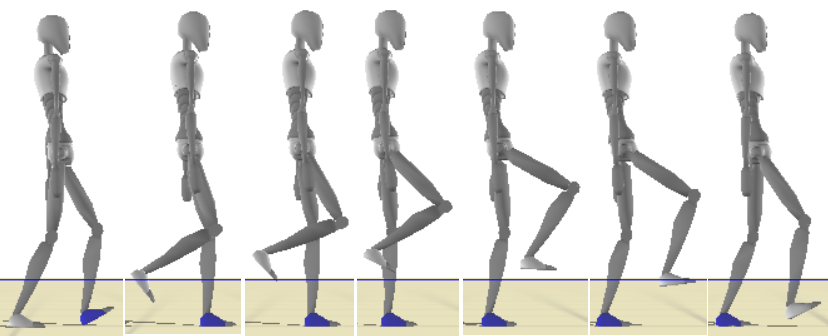
\includegraphics[scale=0.6]{strips/min_drag_25cm.png}
\caption{Marche d'un personnage cherchant à minimiser les forces de résistance du liquide dans 25cm d'eau}
\label{fig:min_drag_25}
\end{figure}


La contrôle de la marche en milieu liquide n'a donc peu été l'objet de travaux dans le domaine de l'animation.  Des travaux aient été réalisés dans le domaine de la biomécanique ne considérant que des cas ou l'immersion dépasse le milieu du torse. En animation, l'utilisation actuelle des systèmes de maintien de l'équilibre limite fortement la capacité à simuler des mouvements variés ce qui empêchant l'émergence de mouvement appropriés au déplacement en milieu liquide. D'autre part, les systèmes de contrôle de la vitesse exposés dans notre état de l'art présentent tous  le défaut de ne pas assurer le suivi correct de la vitesse désirée si l'on s'éloigne des conditions pour lesquels ils ont été optimisés. Enfin, les contrôleurs basé physique implémentant l'interaction avec un fluide ne proposent pas un modèle permettant l'animation d'un modèle humain en temps réel.

Nous proposons grâce contributions. La première contribution est un modèle aquatique permettant de simuler l'influence du liquide sur le déplacement du personnage. La deuxième contribution est un système permettant de combiner plusieurs états nous permettant d'adapter les poses clefs utilisées en fonction de l'environnement et des paramètres spécifiés par l'utilisateur. Notre contrôleur démontre une grande liberté à de spécification de mouvement grâce à une nouvelle gestion de la perte d'équilibre. Enfin, nous améliorons les systèmes utilisant une force virtuelle et modifiant les résultats de l'IPM à l'aide d'un système d'apprentissage autonome permettant ainsi un suivi exact et robuste de la vitesse désirée. 


\begin{figure}[h]
\centering
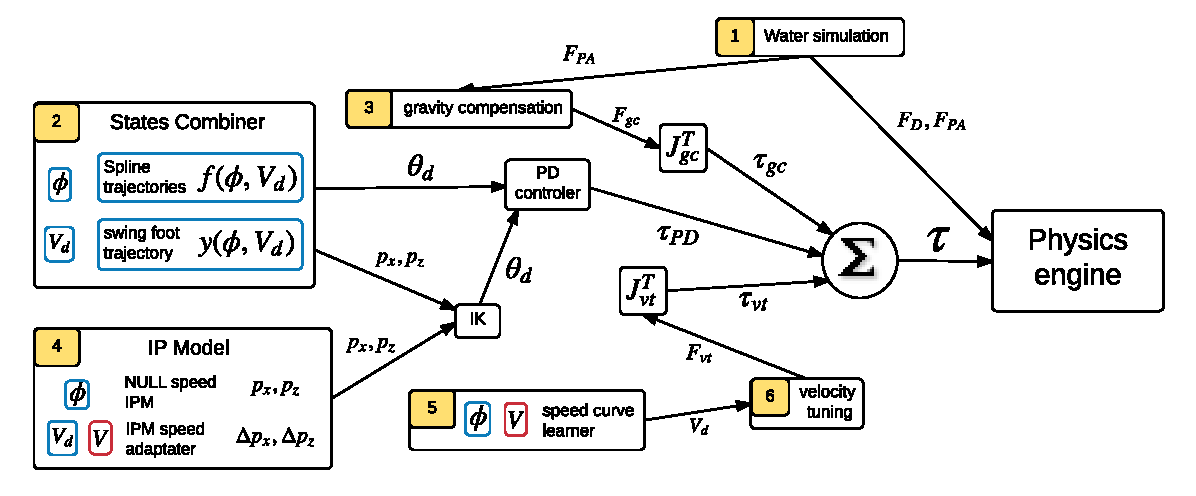
\includegraphics[scale=0.6]{general_process.pdf}
\caption{schéma récapitulatif du contrôleur}
\label{fig:shema_controler}
\end{figure}

\subsection{Vue globale du système}
%


Notre système de contrôle du mouvement est composé de 6 blocs principaux (figure \ref{fig:shema_controler}). Voici une vision globale du fonctionnement du système. 

Nous commençons par calculer les forces résultant de l'influence du fluide sur le personnage. Notre modélisation utilise des formules simples (résistance de l'eau, poussée d'Archimède) nous permettant d'obtenir une simulation en temps réel.

Chaque articulation possède une trajectoire spécifiant les angles à suivre au cours du déplacement. Ces trajectoires sont déterminées à partir de poses clefs définis par l'utilisateur. Les valeurs intermédiaires sont déterminées à l'aide de splines Catmull-Rom. Les trajectoires des articulations de la jambe de balance sont déterminées dynamiquement à partir de la trajectoire désirée pour le pied en phase de vol. La trajectoire du pied en phase de vol est soit spécifiée par l'utilisateur soit déterminée par les systèmes de conservations de l'équilibre lorsque le personnage est dans la phase de descente du pas ou qu'il est en déséquilibre.

Le système de combinaison d'états permet à l'utilisateur de spécifier plusieurs trajectoires pour une articulation chacune d'entre elles étant associée à une vitesse. Le système combinera plusieurs de ces trajectoires pour obtenir un résultat plus adapté à la vitesse désirée. Ce système est particulièrement utile pour les articulations possédant des comportements très différents suivant la vitesse désirée. Les angles lus depuis les trajectoires sont ensuite utilisés par le PD-contrôleur pour calculer les moments à appliquer aux articulations au cours du déplacement.

Nous utilisons un système de compensation de gravité similaire à celui proposé par \cite{coros2010generalized} modifié pour prendre en compte la présence du fluide. Ce système permet de calculer une partie des moments nécessaire au mouvement ce qui nous autorise à utiliser des gains moins élevé dans le PD-contrôleur. L'utilisation de gains faibles est importante pour éviter d'obtenir des oscillations autour de la position désirée et obtenir un résultat s'adaptant plus facilement aux variations de l'environnement.

Le maintien de l'équilibre est obtenu par un placement du pied intelligent obtenu à l'aide d'un modèle de pendule inversé (IPM). Pour permettre l'observation d'un plus grand nombre de styles de marche possible, nous n'utilisons l'IPM seulement lorsque le personnage est dans la phase de descente d'un pas ou lorsque nous détectons une perte de l'équilibre. Pour aider ce système la cheville d'appui possède un modèle de feedback présenté par \cite{yin2007simbicon} corrigeant la position du personnage.

Le contrôle de la vitesse est obtenu à l'aide d'une force virtuelle similaire à celle utilisée par \cite{coros2010generalized}. Ce système a été amélioré pour prendre en compte les variations de vitesse au cours d'un pas. Cette modification nous permet d'obtenir un résultat correspondant plus à la spécification de l'utilisateur. Ce système est aidé par une altération des résultats de l'IPM permettant d'accélérer ou de ralentir le personnage. Ces deux systèmes sont contrôlés par une méthode d'apprentissage et ne nécessitent aucun paramétrage de la part de l'utilisateur.

%
\section{Modèle physique}
\subsection{Modélisation du personnage}
%
\begin{figure}[h]
\centering
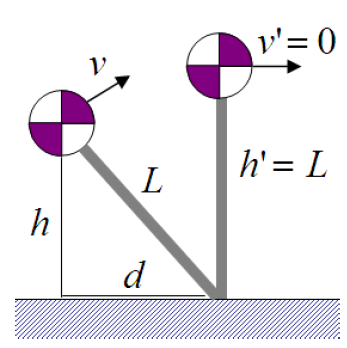
\includegraphics[scale=0.5]{IPM.png}
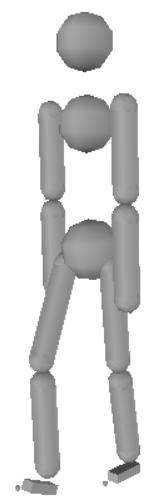
\includegraphics[scale=0.5]{colli_primitives.png}
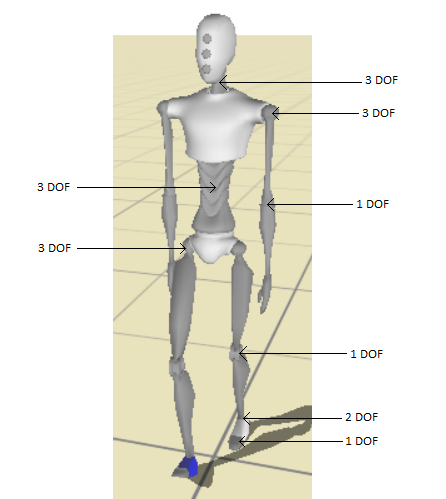
\includegraphics[scale=0.5]{img_dof.png}
\caption{A gauche, modèle du pendule inversé \cite{coros2010generalized}.Au centre, le modèle physique du personnage. A droite, degrés de liberté internes}
\label{fig:ipm}
\label{fig:colli_primitives}
\label{fig:dof}
\end{figure}

Le personnage utilisé est composé de corps solides simples (visible figure \ref{fig:colli_primitives} centre). La tête, le torse, le pelvis et les orteils sont représentés par des sphères. Les bras et les jambes sont représentées par des capsules (cylindre avec des demi-sphères aux extrémités). Les pieds sont modélisés avec des prismes droits. Le squelette est composé des 28 degrés de liberté internes présentés dans la figure \ref{fig:dof} droite plus 6 degrés de liberté externes (position et orientation). Il est intéressant de noter que le poids de chaque membre est modélisé par une valeur et un point d'application qui ne se trouve pas forcément au centre du solide de collision.

%
\subsection{Modélisation des fluides}
%
Lorsque l'on déplace un corps solide à l'intérieur d'un fluide, ce dernier applique trois réactions principales sur le solide. La première est une force de résistance du fluide qui est produite par le déplacement du fluide fluide se trouvant sur la trajectoire du solide. La seconde est une force de friction entre le fluide et le solide. Ces deux réactions du fluide ont pour effet d'entraver le déplacement du solide. La dernière est la poussée d'Archimède, provenant des différences de pression sur la surface du solide, et a pour effet de repousser le solide vers la surface.
Plutôt que de réaliser une modélisation réaliste du fluide (à l'aide des équation de Navier-Stokes par exemple), nous allons baser notre modèle sur la définition d'une hauteur de liquide et les formules de base de dynamique des fluides pour représenter l'influence du liquide sur le personnage. Notre modèle ne considère pas les perturbations du fluide provoquées par le déplacement du personnage. Cette modélisation a l'avantage d'être beaucoup moins couteuse en puissance de calcul ce qui nous permet de conserver une exécution en temps réel tout en permettant une simulation réaliste.
%
\subsubsection{Forces hydrodynamiques}
%
La résistance du fluide est calculée à partir de la formule suivante:
\[
F_D=\frac{1}{2} \rho v^2 A_n C_d
\]


Avec \(C_d\) le coefficient de résistance, \(\rho\) la densité du fluide, \(A_n\) la surface en vue du membre du personnage et \(v\) la vitesse de ce membre. Les surfaces et les vitesses sont calculées à partir de la représentation physique du personnage. La vitesse n'étant pas constante en tout point d'un membre, nous utilisons un découpage en éléments finis de la surface de la représentation physique de chaque membre pour effectuer nos calculs. La surface en vue $A_n$ de chaque élément de surface est calculée en projetant la surface de l'élément dans un plan orthogonal à la vitesse $v$. 

La force finale $F$ à appliquer à chaque élément est calculée en ajoutant la viscosité du fluide à l'aide un coefficient de viscosité $\mu$ 
\[
F=F_D*\mu
\]
Le coefficient de viscosité est obtenu en normalisant la viscosité réelle du fluide par celle de l'eau.
%
\subsubsection{Poussée d'Archimède}
%
La poussée d'Archimède $F_{PA}$ est calculée à l'aide de la formule suivante:
\[
F_{PA}=-V_i \rho g
\]
Le volume immergé \(V_i\) est calculé à l'aide du volume immergé des représentations physiques des différents membres du personnage.  Pour les sphères et les cylindres (jambes et orteils) le volume immergé est calculé en utilisant les formules de géométrie existantes. Pour les prismes droits (pieds) nous découpons le volume en voxels et faisons la somme des volumes des voxels dont le centre se trouve en dessous du niveau de l'eau.
%
\section{Contrôle du mouvement}
%
Notre système se base sur la version du SIMBICON présentée par \cite{coros2010generalized}. Les angles des trajectoires pour les chevilles, le pelvis, le dos et la tête sont spécifiées dans le repère du personnage. Ce repère est équivalant au repère du monde à la différence qu'il est orienté de manière à ce que l'axe z corresponde à la direction que face le personnage. Les angles des trajectoires pour les épaules, les coudes, le genou de la jambe d'appui et les orteils sont spécifiés dans le repère local aux articulations.

Contrairement à \cite{coros2010generalized} nous permettons la spécification manuelle du pied en phase de vol pour permettre l'observation d'un plus grand nombre de style de déplacement. La spécification manuelle est utilisée lors de la phase ascendante d'un pas si le personnage n'est pas en déséquilibre. Cette spécification s'effectue dans le repère local de la hanche en phase de vol.

%
\subsection{Combineur d'état}
\label{sec:multi_state}
%
Suivant la vitesse désirée il est possible que les trajectoires nécessaires pour obtenir un résultat optimal soit radicalement différentes. Par exemple, étudions rapidement le cas de la cheville d'appui. Lorsque le personnage marche vers l'avant il est nécessaire que celui-ci pose le talon en premier. Une fois que le pied est à plat au sol il est nécessaire de conserver un déséquilibre entre les forces appliquées sur l'avant du pied et celles appliquées sur l'arrière du pied pour faire pencher le personnage vers l'avant. Au contraire, pour une marche sur place ou vers l'arrière, il sera nécessaire que celui-ci pose la pointe du pied en premier puis maintienne un déséquilibre des forces le faisant pencher vers l'arrière. chaque type de déplacement (marche vers l'avant, vers l'arrière, sur place, ...) possèdent des caractéristiques spécifique rendant plus facile le mouvement associé. C'est pourquoi nous utilisons une système permettant la définition de plusieurs trajectoires pour les articulations sur lesquelles nous observons ce type de phénomène. Notre système est similaire à celui présenté par \cite{coros2009robust}. Notre système se différencie par deux caractéristiques. Premièrement, contrairement à \cite{coros2009robust} nous n'utilisons pas notre système pour tenter de trouver un état stable en combinant plusieurs états de base. Notre système a pour but de créer une base plus adaptée au suivi de la vitesse désirée. La stabilité étant assurée par l'IPM, le combineur d'états ne cherche pas absolument à produire un état assurant la stabilité par lui-même. La seconde différence est que \cite{coros2009robust} spécifie des états complets (i.e. marche avant, marche arrière, ....). Notre système se contente de capturer les différences ayant une influence importante sur la vitesse. C'est pourquoi nous spécifions plusieurs trajectoires seulement pour les articulations pour lesquelles nous observons des différences importantes suivant la vitesse. De plus notre système a été conçu pour permettre d'utiliser la même trajectoire pour plusieurs vitesses. Nous avons déterminé que les trajectoires possédant des différences significatives sont celles des chevilles, du pelvis, du pied en phase de vol et celle de l'articulation entre le pelvis et le torse (dans une moindre mesure). 

Nous allons maintenant expliquer le fonctionnement du combineur d'états plus en détail. Pour chaque articulation ou système (e.g. pied en phase de vol) possédant plusieurs trajectoires, le combineur d'états va chercher les deux trajectoires associées aux deux vitesses les plus proches de la vitesse désirée. Si la vitesse désirée est inférieure (resp. supérieure) à la vitesse la plus basse (resp. plus haute) spécifiée, le système utilisera directement la trajectoire correspondant à la vitesse la plus basse (resp. haute) comme si il n'y avait qu'une trajectoire définie. Si le système trouve bien deux trajectoires encadrant la vitesse désirée, il créé une nouvelle trajectoire contenant $k$ points clefs répartis de manière uniforme. Lors de nos tests nous avons déterminé qu'un nombre de 10 points clefs était suffisant. Le combineur d'états attribue ensuite des valeurs à chacun de ces points en utilisant une combinaison des valeurs contenues dans les deux trajectoires considérées suivant une loi d'ordre 2:
$$
f(\phi)=f_1(\phi)*\frac{(V_d-V_1)^2}{(V_d-V_1)^2+(V_d-V_2)^2}+f_2(\phi)*\frac{(V_d-V_2)^2}{(V_d-V_1)^2+(V_d-V_2)^2}
$$
Avec $f$ la trajectoire finale,$(f_1,V_1)$ et $(f_2,V_2)$ les deux trajectoires les plus proches de la vitesse désirée.
% 
\subsection{Compensateur de gravité}
Notre système de compensation de gravité se base sur celui présenté par \cite{coros2010generalized}.Nous avons modifié ce système pour permettre la prise en compte d'un milieu liquide. En effet, du fait de la poussée d'Archimède le poids à supporter par le personnage est moins grand lorsqu'il est plongé dans un fluide. De ce fait au lieu de compenser le poids réel de chaque membre du personnage, il faut compenser le poids effectif (poids observable dans le fluide). Notre modification consiste donc à calculer la force résultant de la poussée d'Archimède sur chaque membre du personnage et de soustraire celle-ci à la force virtuelle à appliquer. Il parait intéressant de noter qu'il ne suffit pas simplement de diminuer l'intensité de la force à appliquer. En effet suivant la modélisation des membres du personnage, il est fréquent que la densité soit variable à l'intérieur de ceux-ci. Par exemple, dans notre modélisation seul les bras possèdent une densité uniforme. De ce fait le point d'application de la force  $F_{gc}$ compensant la gravité et celui de la force $F_{PA}$ causée par la poussée d'Archimède seront différent, ce qui nous oblige à déterminer le point d'application de la force finale $F$:
$$
F=F_{gc}- F_{PA}
$$

Si le milieu est assez dense il est fortement possible que les membres du personnage disposant d'une densité faible aient un poids plus faible que la force causée par la poussée d'Archimède. Dans ce cas le système génère des moments ayant pour effet de baisser les membres du personnage au lieu de les lever. Nous ne traitons pas ce cas comme un cas particulier. En effet, comme dit précédemment le but du compensateur de gravité est de calculer une partie des moments nécessaires pour pouvoir se rapprocher de la position désirée. Or si nous avons une poussée d'Archimède plus forte que le poids des membres du personnage, ceux-ci essaierons de flotter ce qui entraverait le déplacement du personnage. Il est donc intéressant de conserver le système présenté ci-dessus même dans ce cas particulier car il aidera tout de même le personnage à suivre les poses désirées.
%.
\subsection{Conservation de l'équilibre}
%
L'équilibre du personnage est obtenu par le placement intelligent du pied à l'aide d'un modèle de pendule inversé (IPM) et de fonctions de feedback sur certaines articulations (balance feedback). Les systèmes de contrôle de vitesse (section \ref{sec:speed_control}) permettent également un maintien de l'équilibre du fait qu'ils maintiennent le système autour d'une vitesse stable. 
%
\subsubsection{Modèle du pendule inversé}
%
\label{sec:IPM}
L'utilisation d'un IPM permet d'avoir un système efficace de conservation d'équilibre ne nécessitant pas de paramétrage de l'utilisateur. Dans le cadre de notre  projet nous utiliserons un IPM similaire à celui présenté par \cite{coros2010generalized}. Le système utilise un IPM supposant une position nulle à la position verticale et une longueur de jambe constante. 


Bien que l'IPM soit intéressant il limite les possibilités de mouvement. Par exemple il rend impossible un mouvement définissant une trajectoire rectangulaire pour le pied comme l'on voit sur la figure \ref{fig:min_drag_25}. Ce genre de déplacement est important dans le cadre de notre étude car elles sont typiques d'environnement ou le mouvement est beaucoup entravé (par exemple de la neige). Pour permettre l'observation de tels déplacements nous avons rajouté la possibilité de manuellement définir la position du pied au cours du pas. Cette définition manuelle est considérée temps que le personnage est dans la phase ascendante du pas \(V_{COM}(y)>0\) et qu'il n'est pas dans un état instable. Nous déterminons une instabilité du personnage si nous détectons une variation irrégulière du motif de vitesse observé au cours d'un pas (voir la section \ref{sec:speed_virt_force}). Si un état instable est détecté nous utilisons le résultat de l'IPM pour la totalité du pas jusqu'à ce que nous retournions dans un état stable.
%

%
\subsection{Contrôle de vitesse}
%
\label{sec:speed_control}
Dans le cadre de ce projet, la capacité à marcher à une vitesse donnée est un critère primordial. De plus nous souhaitons obtenir un système qui sera robuste à la variation du milieu. C'est à dire que nous souhaitons que notre contrôler soit capable de marcher dans un mètre d'eau ou dans 50cm d'huile aussi bien que lorsqu'il ne se trouve pas en présence d'un fluide. Pour obtenir un tel résultat, nous utilisons une force virtuelle ainsi qu'un système d'altération des résultats de l'IPM.
%
\subsubsection{Contrôle de vitesse par force virtuelle}
%
\label{sec:speed_virt_force}

Pour obtenir une vitesse désirée nous allons appliquer une force virtuelle horizontale qui accélèrera ou ralentira le personnage en déplaçant le centre des masses. De manière similaire à \cite{coros2010generalized} nous utilisons un PD-contrôleur utilisant l'écart entre la vitesse désirée et la vitesse actuelle du personnage pour calculer la force virtuelle nécessaire.
Cependant la chaine de membres du personnage considérés pour l'application de la force est la chaine reliant le torse au pied d'appui (donc ne prend pas en compte la tête du personnage). La raison de ce choix est qu'il ne parait pas naturel de pencher la tête si l'on veut aller dans une direction. Les valeurs utilisées pour la jacobienne sont différentes de celles utilisées par \cite{coros2010generalized}. Nous utilisons la somme des vecteurs séparant les articulations pondérés par le poids du membre présent entre ces deux articulations.
\[
J_n ^T (p)=\frac{1}{M}\sum_{\substack{0<i\leq n}} ((P_i(x,y,z)-P_{i-1}(x,y,z))*M_i)
\]
Avec \(M\) la somme des poids de tous les membres considérés par le système et \(P_i(x,y,z)\) la position de l'articulation \(i\) de la chaine, \(P_0(x,y,z)\) étant le point d'application de la force. Cela évite que les articulations du bas du corps reçoivent une grande importance du fait quelles se trouvent loin du torse (qui représente une grande partie de la masse du personnage). Cette caractéristique est intéressante car un moment appliqué sur la cheville ayant pour but de faire pencher le torse aurait de grande chance de se faire annuler par un moment sur la hanche ou le pelvis ayant pour but de redresser le personnage. De plus il est plus simple de créer un déséquilibre régulier du personnage en appliquant un moment sur l'articulation entre le pelvis et le torse qu'en appliquant un moment sur la cheville ce qui renforce l'idée que le torse doit bien être considéré indépendamment du bas du corps.

Il est facile d'observer que la vitesse de déplacement du centre des masses n'est pas constant au cours d'un pas. De ce fait l'application d'une force virtuelle se basant sur une vitesse désirée constante aura pour effet de faire disparaître ce phénomène, voire demander localement au personnage de ralentir alors que l'on voudrait le voir accélérer de manière globale. C'est pourquoi il serait plus intéressant d'appliquer une force constante au cours d'un pas. Cependant ce genre de force constante serait difficile à déterminer et diminuerait la robustesse du modèle car elle ne pendrait pas en compte les évènements se passant au cours d'un pas (i.e. ralentissements du au contact avec un objet par exemple). On peut observer que lorsque nous sommes dans le cas d'un déplacement stable, ces variations de vitesse sont constantes à chaque pas. L'idée serait donc d'adapter la vitesse désirée que l'on communique au PD-contrôler suivant les variations de vitesse observées au cours du pas. C'est pourquoi nous avons construit un système permettant d'apprendre cette courbe de variations de vitesse de manière à appliquer une force virtuelle plus adaptée. De manière similaire aux trajectoires des articulations, cette courbe est définie comme une fonction de la phase \(\phi\) et possède un nombre de point de référence pouvant être définis par l'utilisateur. Les valeurs entre les points de références sont également déterminées à l'aide de splines Catmull-Rom. Un nombre de 10 points de référence s'est montré être suffisant pour permettre l'obtention d'une courbe précise tout en évitant de surcharger le système. Le système utilise une courbe pour la vitesse suivant l'axe sagittal et deux courbes pour l'axe coronal (une pour chaque phase d'appui). L'axe coronal nécessite deux courbes car dans le cas d'une vitesse non nulle selon l'axe coronal le mouvement observé devient asymétrique.Une autre différence entre les deux axes et que pour l'axe coronal nous stockons directement les vitesses en $m.s^{-1}$ alors que pour l'axe sagittal nous stockons des facteurs multiplicateurs à appliquer à la vitesse désirée par l'utilisateur. L'utilisation des facteurs multiplicateurs nous permet une plus grande aisance à nous adapter aux variations de vitesses demandées par l'utilisateur. En effet pour une variation de vitesse de moyenne amplitude il est fortement possible que la courbe de facteurs multiplicateurs reste identique. Cependant vu que nous travaillons généralement avec une vitesse nulle suivant l'axe coronal, il nous est impossible de nous baser sur un coefficient multiplicateur.

\begin{figure}[h]
\centering
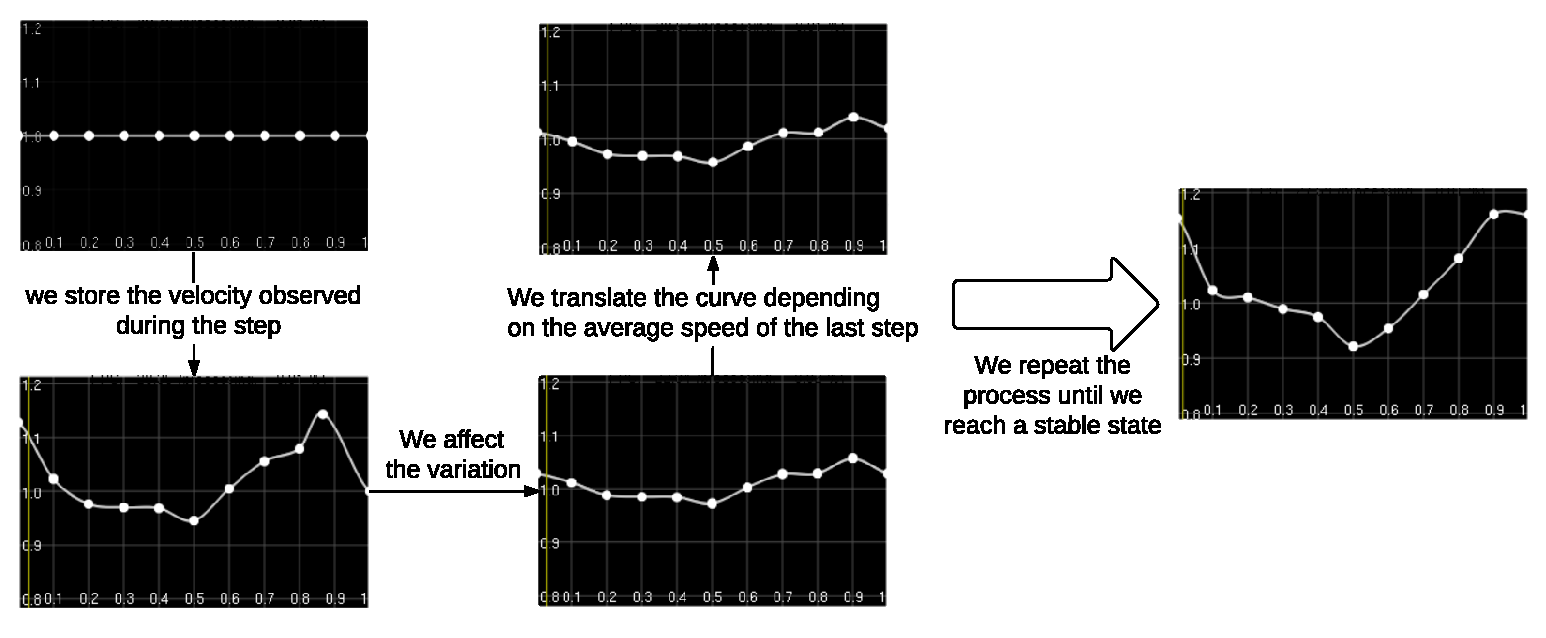
\includegraphics[scale=0.45]{speed_curve_learner.pdf}
\caption{Schéma présentant le processus d'apprentissage de la courbe de vitesse}
\label{fig:speed_curve_learner}
\end{figure}


Ce paragraphe explique de manière plus précise l'apprentissage des courbes de vitesse. Comme présenté sur le schéma \ref{fig:speed_curve_learner} le système d'apprentissage des courbes de vitesse s'effectue par une boucle de 3 étapes répétées jusqu'à l'obtention d'une courbe stable. La première étape est de relever, aux cours d'un pas, la vitesse réellement observée pour chaque point de référence. Une fois le pas terminé nous calculons la variation moyenne entre la courbe que nous avions et la courbe observée. La deuxième étape consiste à, si la variation moyenne observée est inférieur à un seuil, adapter les valeurs stockées pour les rapprocher des valeurs observées. Nos tests ont montré qu'un seuil de 0,4 donne des résultat satisfaisant. Nous notons tout de même qu'il peut être intéressant d'utiliser une heuristique plus élevée au début de la phase d'apprentissage car il est possible que la trajectoire initialement utilisée et très différente de la trajectoire observée.  Pour éviter d'obtenir d'oscillations autour de la courbe vers laquelle on cherche à converger, la variation de chaque point est limitée à une variation d'au maximum la valeur de la variation moyenne constatée. Pour finir nous modifions les points de la courbe de façon à ce que la nouvelle courbe définisse les valeurs à demander pour obtenir la vitesse voulue. Pour obtenir ce résultat nous déterminons le ratio entre la vitesse moyenne demandée et la vitesse moyenne observée lors du dernier pas et nous multiplions tout les points de la courbe par ce ratio. Dans le cas de l'axe coronal nous utilisons le ratio entre la vitesse demandée et la moyenne des vitesses observées lors des deux derniers pas.

La présence du seuil nous permet de détecter les variations irrégulières de la courbe de vitesse. Une fois la situation d'équilibre atteinte nous obtenons une courbe stable qui est caractéristique au déplacement observé. Si l'on constate une variation de cette courbe cela veut dire qu'un élément est venu perturber le déplacement. Dans ce cas, nous déclarons au contrôleur que nous ne sommes plus dans un état stable ce qui signale au contrôleur qu'il doit utiliser l'IPM durant toute la durée du pas jusqu'à ce que le mouvement redevienne stable. Une fois le mouvement redevenue stable, c'est à dire que la variation moyenne de la vitesse est redevenue inférieure à l'heuristique, nous recommençons à utiliser le système décrit précédemment pour adapter la courbe de vitesse. Si le système détecte plus de 5 pas consécutif pour lesquels le mouvement est déclaré instable, alors nous réinitialisons tous les points des courbes de vitesses à la valeur de la vitesse désirée spécifiée par l'utilisateur. Cela nous permet de restaurer le système dans le cas où les courbes auraient subi une variation très forte les éloignant trop de la courbe résultant de l'IPM ce qui bloque le système.
%
\subsubsection{Altération des résultats de l'IPM}
\label{sec:ipm_alt}
%
Bien que le système utilisant une force virtuelle pour contrôler la vitesse permette un réglage fin de la vitesse, il ne permet pas d'effectuer de grandes variations de vitesses. En effet, pour réaliser de telles variations nous aurions besoin d'une force virtuelle très importante ce qui aurait des effets indésirables. En effet une force virtuelle élevée provoquerait l'apparition de moments très élevés. Si les moment maximaux aux articulation on été  paramétrés alors les variations de la force virtuelle n'auront plus d'impact sur le personnage et il serait possible d'observer un mouvement peu naturel si seules certaines articulation de la chaine de membres affectés ont atteint leur maximum. Les les moment maximaux n'ont pas été définis alors une force élevée résulterait en des phénomène non réalistes. Pour régler ce problème \cite{coros2010generalized} propose d'altérer les résultats de l'IPM pour aider à atteindre la vitesse voulue. Cependant, cette modification est basée sur une relation linéaire dépendant de la vitesse désirée. Cette relation linéaire rend le système trop peu efficace notamment pour des mouvements dans un fluide qui ralentira le personnage.

Vu qu'il semble impossible d'utiliser une simple loi dépendant de la vitesse désirée, nous avons décidé d'utiliser un système qui stocke un $\Delta(x,z)$ qui sera ajouté au résultat de l'IPM. Pour pouvoir déterminer la valeur de ce $\Delta$ nous utilisons une méthode incrémentale. A la fin de chaque pas nous utilisons un PD-contrôleur se basant sur la différence entre la vitesse désirée et la vitesse réellement observée au cours du pas pour déterminer comment doit évoluer le $\Delta(x,z)$ pour permettre au personnage de se déplacer à la vitesse désirée. Nous n'utilisons ce système que sur l'axe sagittal. Les vitesses demandées sur l'axe coronal étant plus faibles le personnage n'a pas besoin de ce système pour les atteindre.

Ce système de contrôle de vitesse est extrêmement efficace et robuste. Cependant, si l'on utilise un $\Delta(x,z)$ trop élevé dans le but d'accélérer le personnage cela risque d'empêcher l'IPM de maintenir l'équilibre. C'est pourquoi nous avons mis une limite aux valeurs du $\Delta(x,z)$. Nous fixons cette valeur à 0,09m, ce qui correspond à la valeur maximale permettant de conserver l'équilibre avec un personnage immergé jusqu'à la taille dans de l'eau, les autres situations de test supportant des valeurs plus élevées cela parait être une bonne sécurité. 
%

\subsection{Optimisation hors ligne}
%
Le nombre très important de paramètres que prend le système en entrée rend très difficile la recherche manuelle d'une solution optimale à un problème. C'est pourquoi ce travail de recherche est effectué à l'aide d'un système d'optimisation hors ligne. Le principe est d'explorer l'espace des paramètres et conserver la "meilleure solution" trouvée. La notion de "meilleure solution"  est définie à l'aide d'une fonction objectif qui permettra d'évaluer la qualité de chaque ensemble de paramètres. Par exemple, il est possible de faire la somme des moments appliqués aux articulations durant un certain temps pour obtenir une fonction évaluant l'énergie dépensé par le personnage. L'exploration de l'espace des paramètres peut se faire de manière aléatoire, mais il est plus rapide d'utiliser un algorithme tel que la descente de gradient. L'optimisation hors ligne permet donc d'obtenir un mouvement optimal pour les critères définis dans la fonction d'évaluation. Ce qui veut dire que le mouvement obtenu possèdera des caractéristiques propres à la fonction d'évaluation qui a été utilisée.


Les paramètres que nous optimiserons sont la trajectoire du pied en phase de vol (positions) et les trajectoires angulaires associées aux éléments suivants:
\begin{itemize}
\item{le pelvis;}
\item{l'articulation du dos;}
\item{la cheville d'appui;}
\item{la cheville en phase de vol;}
\item{le genou d'appui;}
\end{itemize}

Nous n'optimisons pas les articulations des bras et du cou de manière à obtenir un modèle à partir duquel un utilisateur peut spécifier des actions utilisant ces membres. Nous n'optimisons pas non plus les gains des différents PD-contrôleurs. Nous utilisons des gains qui ont été génériques*réécrire*

%
\subsubsection{Fonction objectif}
%
Nous allons construire notre fonction d'optimisation $f_{eval}$ en utilisant d'une part une combinaison pondérée de critères d'évaluation représentant un but physique et d'autre part des heuristiques. Notre fonction d'évaluation se base sur trois critères 
\begin{equation}
f_{eval}=\sum_{\substack{t}} (\alpha f_{energ} + \beta f_{acc} + \gamma f_{drag})
\label{eq:simple_objective}
\end{equation}
Chacune des $f_i$ est normalisée par la valeur moyenne obtenue en effectuant une série optimisation du système en utilisant uniquement la fonction $f_i$ comme fonction d'évaluation. Les poids $\alpha$, $\beta$, $\gamma$ nous permettent de choisir facilement l'importance qu'aura une composante dans le résultat final. Les critères d'évaluation que nous utilisons sont les suivants:
\begin{itemize}
\item{\textit{Minimisation de l'énergie} ($f_{energ}$). Le but de ce critère est de faire tendre le résultat vers une simulation utilisant le minimum d'énergie dépensé par le personnage. Cela nous permettra d'éviter les mouvement superflus. Ce critère calculé par la calcul par le calcul de la somme des moments aux articulations $f_{energ}=\sum_{\substack{i}}{\tau_i}$} 
\item{\textit{Minimisation de la résistance de l'eau}. ($f_{drag}$) Ce critère aura pour effet de favoriser les mouvements du personnage effectués hors de l'eau et de chercher des trajectoires évitant les pics de vitesses en dessous de l'eau. Ce critère est calculé par la somme des moments produits par la force de résistance de l'eau sur chacune des articulations . Ces moment sont calculé par le produit vectoriel entre les force de résistance de l'eau et le vecteur allant de l'articulation au point d'application de la force; $f_{energ}=\sum_{\substack{i}}\sum_{\substack{j}}((P_j(x,y,z)-P_i(x,y,z)) \otimes  F_j)$ avec $P_j(x,y,z)$ le point d'application de la force et $P_i(x,y,z)$ la position de l'articulation affectée.}
\item{\textit{Minimisation des accélérations angulaires} ($f_{acc}$). Notre but est de parvenir à obtenir un mouvement et des trajectoires à reproduire lisses. Lors de test préliminaires nous avons observé des fortes variations dans les positions désirées pour certaines articulations (i.e. la cheville d'appui). Ceci nous fait penser que la méthode d'évolution avait apprit des détails optimisant le mouvement mais le rendant moins robuste. En introduisant ce critère nous voulons minimiser ces détails pour rendre le contrôler plus robuste. Ce critère est calculé par la somme des accélérations angulaires des poses désirées $\ddot{\theta_d}_i$ et de celles du mouvement observé $\ddot{\theta}_i$.  Pour donner une plus grande importance au mouvement final avons attribué une pondération de 0.25 aux accélérations des poses désirées et une pondération de 0.75 aux accélérations du mouvement observé: $f_{acc}=0.25*\sum_{\substack{i}}\ddot{\theta_d}_i+0.75*\sum_{\substack{i}}\ddot{\theta}_i$ }
\end{itemize}

Comme nous l'avons expliqué lors de la présentation des systèmes de contrôle de vitesse (section \ref{sec:ipm_alt}), l'utilisation de valeurs élevées pour l'altérateur d'IPM peut rendre le mouvement instable. De plus, ce système entraine une modification majeure des résultats de la simulation (en général il raccourci les pas du personnage). Lors de nos premières évaluations nous avons remarqué que l'altérateur d'IPM permettait d'obtenir la vitesse spécifiée même si les poses clefs ne sont pas adaptées. C'est pourquoi nous avons ajouté une une pénalisation de ce système. De cette façon la stratégie d'optimisation apprendra des poses clefs ne se reposant pas sur l'altérateur et il ne sera utilisé que lorsqu'il est impossible de suivre la vitesse désirée sans s'en servir. Cette pénalisation est représenté par une augmentation de la fonction d'évaluation par un facteur multiplicateur de $(1+0.1*\frac{\Delta(x,z)}{max(\Delta(x,z))})$, avec $\Delta(x,z)$ la valeur de l'altérateur à l'état d'équilibre et $max(\Delta(x,z))$ la valeur maximale autorisée (0.09). Nous obtenons donc la fonction objectif suivante:
$$
f_{eval}() = \sum_{\substack{t}} (\alpha f_{energ} + \beta f_{acc} + \gamma f_{speed})*(1+0.1*\frac{\Delta(x,z)}{max(\Delta(x,z))}) 
$$

Enfin nous ajoutons des heuristiques nous autorisant à définir les limites strictes des solutions que nous acceptons:
\begin{itemize}
\item{\textit{vérification de la vitesse} ($f_{speed}$). Bien que nous disposons de systèmes nous assurant que la vitesse spécifiée sera la vitesse respectée (section \ref{sec:speed_control}), il est possible que l'optimisation arrive à trouver des combinaisons de paramètres qui rendent la convergence vers la vitesse désirée très longue voire impossible (par exemple si l'on a une vitesse positive avec des paramètres pour aller vers l'arrière). Cette heuristique est représentée par une pénalisation très élevée si la vitesse courante et la vitesse désirée excède 1\% de la vitesse désirée: si $||V-V_d||>0.01*||V_d||$ alors $f_{speed}=10^{10}$}
\item{\textit{stabilité du mouvement} ($f_{balance}$).  Cette heuristique sert à nous assurer que nous nous trouvons bien dans un état stable, c'est à dire un état utilisant la spécification désirée du pied en phase de vol pour le début du pas. Cette heuristique est représentée par une pénalisation très élevée si l'on détecte un pas pour lequel le mouvement est déclaré instable alors $f_{balance}=10^{15}$  }
\end{itemize}
 La version complète de notre fonction objectif est donc:

\begin{equation}
f_{eval}() =\sum_{\substack{t}} (\alpha f_{energ} + \beta f_{acc} + \gamma f_{speed})*(1+0.1*\frac{\Delta(x,z)}{max(\Delta(x,z))}) + f_{speed} + f_{balance}
\label{eq:complete_eval}
\end{equation}



%
\subsubsection{Méthode d'évolution des paramètres}
Nous nous trouvons dans le cas d'un système espace complexe de variables avec de nombreux minimum locaux. De manière similaire à de nombreux articles concernant l'animation basée physique (*citer 3/4 articles*) nous utiliserons la méthode de "covariance matrix adapation" (CMA) \cite{hansen2006cma} pour explorer l'espace des solutions. CMA est une méthode d'évolution cherchant à apprendre la matrice de covariance de l'espace de recherche à l'aide d'un échantillonnage aléatoire.



%%%%%%%%%%%%%%%%%%%%%%%%%%%%%%%%%%%%%%%%%%%%%%%%
%%%%%%%%%%%%%%%%%%%%%%%%%%%%%%%%%%%%%%%%%%%%%%%% 

%
\section{Résultats}
%
\subsubsection{Implémentation}
Le moteur physique utilisé est "Open Dynamics Engine" (ODE). La simulation physique s'effectue selon un pas de temps de 0,0005s. Seul le modèle humain présenté précédemment est utilisé pour les tests. Les collisions entre les différentes parties du personnage ne sont pas prises en compte. Les gains des PD-contrôler utilisés sont repris des fichiers de configurations de travaux précédents \cite{coros2009robust}. La modélisation physique du personnage est également identique à celle utilisée par \cite{coros2009robust}. Les moments aux articulations sont limités à $|\tau|<200Nm$ pour les hanches et les genoux et à $|\tau|<100Nm$ pour les autres articulations.
Les simulations sont effectuées avec une implémentation en single-thread sur une machine disposant de 8Go de mémoire RAM et une processeur i5 2.5GHz.

La présentation de nos résultats s'organise suivant deux étapes. La première consiste à effectuer plusieurs optimisations en utilisant différentes combinaisons de poids dans la fonction d'évaluation. Nous commencerons par étudier l'impact de chaque fonction objectif élémentaire \ref{eq:simple_objective}. Puis nous étudierons plusieurs compositions versions de la fonction d'optimisation. La seconde sera d'utiliser la combinaison que nous estimerons comme optimale pour créer un contrôler pouvant supporter les variations de vitesse désirée et les variations de niveau de fluide. Nous testerons ensuite la robustesse de ce contrôler à l'application de forces externes et le changement de vitesse coronale.

\subsection{étude de la fonction d'évaluation}

Durant cette partie nous effectuerons pour chaque version de la fonction d'évaluation 5 simulations. Chaque simulation sera effectuée un niveau de liquide différents. Les niveau de liquides étudiés sont 0, 0.25, 0.5, 0.75 et 1 (les valeurs sont en mètres). Nous effectuerons nos simulations dans un liquide équivalent à de l'eau (masse volumique $\rho =1000kg.m^{-3}$ et coefficient de viscosité  $\mu =1$). Sauf contre indication les simulations sont effectuées pour une vitesse de $0.7m.s^{-1}$. Nous étudions d'abord l'influence de chaque critère d'optimisation sur le mouvement.

\subsubsection{Étude de la minimisation de l'énergie}

\begin{figure}[h]
\centering
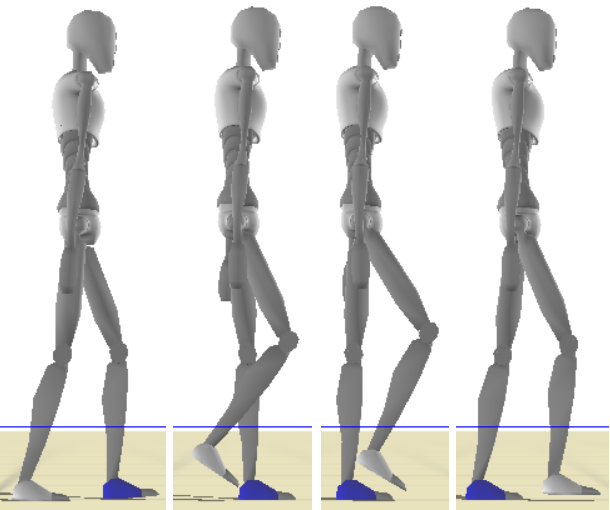
\includegraphics[scale=0.37]{strips/min_torque_25cm.png}
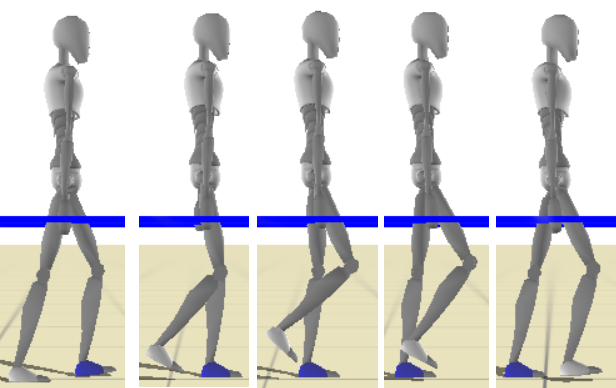
\includegraphics[scale=0.5]{strips/min_torque_75cm.png}
\caption{Marche d'un personnage cherchant à minimiser l'énergie dépensée du liquide dans 25cm d'eau (gauche) et dans 75cm d'eau (droite)}
\label{fig:min_energ}
\end{figure}


Cette version ne prend en compte que la composante cherchant à minimiser l'énergie dépensée par le personnage. Les résultats que nous attendons est sont des mouvements cherchant à rester un maximum au fond de l'eau.

Comme nous nous y attendions le personnage lève très peu le pied en phase de vol lorsque le niveau d'eau est faible \ref{fig:_energ} (gauche). Nous remarquons tout de même une augmentation de la hauteur des pas dès que le niveau d'eau atteint les genoux \ref{fig:_energ} (droite). *mettre expliquation hypothétique?*

\subsubsection{Étude de la minimisation de la résistance de l'eau}

\begin{figure}[h]
\centering
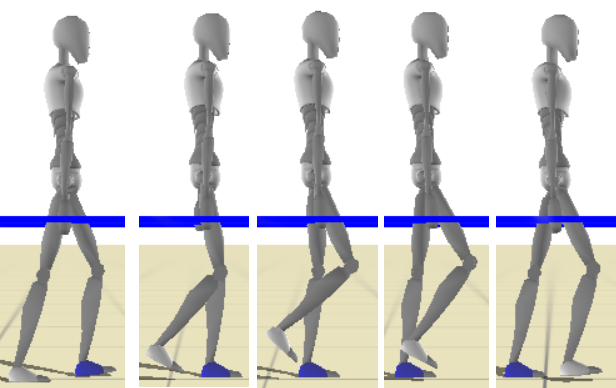
\includegraphics[scale=0.5]{strips/min_torque_75cm.png}
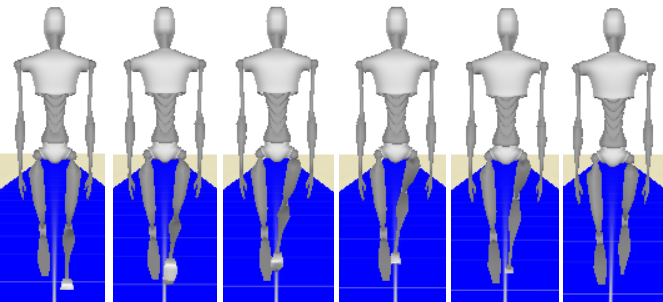
\includegraphics[scale=0.37]{strips/min_drag_25cm_from_back.png}
\caption{Marche d'un personnage cherchant à minimiser l'opposition du liquide au mouvement dans 75cm d'eau (gauche) et dans 25cm d'eau vue de dos (droite) *Attention l'img de droite n'est pas la bonne car je n'ai pas encore le controler du 75cm pr le drag*}
\label{fig:min_drag2}
\end{figure}

Cette version ne prend en compte que la composante cherchant à minimiser la l'effet de la résistance de l'eau. Cette version ne prenant en compte que le drag cela veux dire que pour une hauteur d'eau de 0 la fonction d'évaluation est inutile, ce qui fait que nous n'étudierons donc pas ce cas. Les résultats que nous attendons est sont des mouvements cherchant à éviter un maximum le contact avec l'eau, donc un personnage cherchant à sortir le jambes de l'eau. On s'attend à apercevoir qu'après un certain niveau d'eau il devient impossible de sortir les jambes de l'eau et donc le personnage cherche à effectuer des mouvements les moins amples et les moins rapides possible dans l'eau. 
 
Comme nous nous y attendions le personnage cherche bien à sortir le pied en phase de vol de l'eau \ref{fig:min_drag_25}, ce phénomène est déjà presque impossible à une hauteur de 0,5m. Au dessus de 0,5m le contrôle choisit de ne plus lever la jambe et cherche à obtenir le mouvement optimal en restant au fond du liquide  \ref{fig:min_drag_25} (gauche). Il est également intéressant de noter que le personnage cherche à aligner le tibias avec le sens du déplacement pour éviter que l'eau applique une résistance dessus. Ce phénomène est particulièrement remarquable dans la phase de levée du pied. Pour les niveau d'eau ou le personnage cherche à sortir le pied hors de l'eau on remarque que le pied a une trajectoire assez courbée vers l'intérieur du personnage  \ref{fig:min_drag2} (droite). Ce phénomène doit probablement servir à lever le pied aussi haut que possible mais il ne donne pas un résultat visuellement réaliste.  

\subsubsection{Minimisation des accélérations angulaires}
Cette version ne prend en compte que la composante pénalisant les accélérations élevées. Nous nous attendons à trouver un résultat proche de ceux obtenus pour $f(1,0,0)$. En effet, obtenir des accélérations élevée demanderait des torques élevés. La différence que nous attendons principalement est au niveau de la trajectoire désirée de la cheville d'appui. Nous nous attendons à un résultat ayant bien moins de variations.

Comme prévu on remarque que les résultats sont très similaires à ceux obtenus pour $f(1,0,0)$. Le personnage conserve le pied tellement près du sol que même une faible variation du milieu provoque une chute du personnage du fait d'un contact prématuré du pied en phase de vol avec le sol. Contrairement à ce que nous espérions nous observons toujours des variations assez importante sur la trajectoire de la cheville d'appui. Cela veux dire que ces variations on un importance plus grande que ce que nous pensions.

Maintenant nous allons étudier quelques combinaisons de la fonction d'évaluation \ref{eq:complete_eval}  Nous utiliserons la dénomination suivante lorsque nous voulons nous référer à une des combinaison $f(\alpha,\beta,\gamma)$. Dans cette partie nous ne réétudierons pas les niveaux d'eau pour lesquels les résultats étaient similaires pour les trois critères d'optimisation (0, 0.75 et 1) car une combinaison des résultat donnerais de toute façon le même résultat. Donc nous n'étudierons que les niveau d'eau suivants 0,25 et 0,5. Le but de cette étude et de trouver une combinaison permettant d'obtenir un mouvement fortement conditionné par la présence du liquide, dépensant une quantité d'énergie assez faible et ne présentant pas d'accélérations brusques.

\subsubsection{étude de f(2,8,1)}

\subsubsection{étude de f(3,6,1)}

\subsubsection{étude de f(4,5,1)}

*faire un comparatif visuel des mouvement obtenus suivant le niv d'eau pr les diff combinaisons d'évaluations*
*faire une comparaison en désactivant les systèmes créés*
*si il y en a présenter les trucs qui peuvent être utilisé en tant que feed back*
*faire une partie limitation*

\subsection{étude du contrôleur complexe}

\section{Conclusion}
%
*faire une conclusion qui contient la partie travaux futur*
%



%
\nocite{*}
\bibliographystyle{splncs03}
\bibliography{references}
%
\newpage
\section{Annexe}
\end{document}
